\documentclass[conference]{IEEEtran}
\IEEEoverridecommandlockouts
% The preceding line is only needed to identify funding in the first footnote. If that is unneeded, please comment it out.
\usepackage{cite}
\usepackage{amsmath,amssymb,amsfonts}
\usepackage{tabularx}
\usepackage{algorithmic}
\usepackage{graphicx}
\usepackage{textcomp}
\usepackage{xcolor}
\usepackage{tikz}
\usepackage{multirow}
\usetikzlibrary{positioning}
\usepackage{hyperref}

\def\BibTeX{{\rm B\kern-.05em{\sc i\kern-.025em b}\kern-.08em
    T\kern-.1667em\lower.7ex\hbox{E}\kern-.125emX}}
\begin{document}

\title{Retrieval-Augmented Generation in System Logs Context \\
}

\author{\IEEEauthorblockN{Nurbek Bolat}
\IEEEauthorblockA{\textit{Department of Business} \\
\textit{Univ. of Europe for Applied Sciences}\\
Potsdam 14469, Germany \\
nurbek.bolat@ue-germany.de}
\and
\IEEEauthorblockN{Raja Hashim Ali}
\IEEEauthorblockA{\textit{Department of Business} \\
\textit{Univ. of Europe for Applied Sciences}\\
Potsdam 14469, Germany \\
hashim.ali@ue-germany.de}
}

\maketitle

\begin{abstract}
Retrieval-Augmented Generation (RAG) is a powerful approach that enhances language models by integrating retrieval mechanisms into their generation pipelines. As systems increasingly rely on log data for monitoring and diagnosis, leveraging RAG to interpret logs offers new opportunities in intelligent automation and observability.

Current solutions in log analysis rely heavily on static search and pattern-matching methods, lacking semantic understanding or contextual relevance. Furthermore, integrating RAG in real-time log systems remains relatively unexplored, particularly using efficient lightweight models suitable for deployment in resource-constrained environments.

In this study, we implemented a RAG-based log interpretation system using a monorepo architecture powered by TurboRepo, combining a NestJS backend and Angular frontend. We utilized TinyLLaMA as the core language model and dynamically constructed prompts using sliced segments from system log files.

Our experiments show that the system provides context-aware responses to log queries with low latency and high relevance. Additionally, the integration supports efficient scaling and deployment.

This work contributes a novel RAG framework tailored for log data and lightweight environments, opening avenues for real-time, explainable log intelligence in production-grade applications.
\end{abstract}

\begin{IEEEkeywords}
Retrieval-Augmented Generation, Log Analysis, TinyLLaMA, NestJS, Angular, TurboRepo, Monorepo Architecture
\end{IEEEkeywords}

\section{Introduction}

The exponential growth in system complexity has led to an increased reliance on logs for debugging, performance monitoring, and security auditing. Logs provide a chronological trace of events that reflect the behavior and state of systems, making them essential for engineers and analysts.

However, extracting insights from logs remains a non-trivial task, particularly when the volume, velocity, and variety of log data exceed human analysis capabilities. Traditional log management approaches often rely on rule-based parsing, keyword search, and pattern-matching, which lack semantic depth and adaptability. As artificial intelligence progresses, integrating natural language models into log analysis workflows presents a promising direction.

Recent advances in language models and Retrieval-Augmented Generation (RAG) architectures have enabled more context-aware responses to natural language queries \cite{lewis2023ragqa}. By combining prompt-based generation with targeted retrieval from relevant data sources, these systems bridge the gap between static information and dynamic reasoning. In this study, we extend this idea to system log files.

Our work leverages a monorepo implementation using TurboRepo to combine a NestJS backend and Angular frontend. The backend integrates TinyLLaMA, a lightweight transformer-based language model, which receives sliced log segments appended to the prompt, thus providing context for accurate responses. The aim is to assist developers or operators by interpreting logs automatically and answering user queries with minimal latency.

The resulting system provides a lightweight, production-friendly, and scalable solution for real-time log understanding. This paper presents the methodology, architecture, and evaluation of this approach, highlighting both its practicality and potential for broader adoption in infrastructure monitoring, observability, and DevOps automation.

\subsection{Related Work}

A wide body of literature exists in the domain of log analysis and anomaly detection. Traditional techniques such as DeepLog \cite{du2020deeplog} and LogAnomaly \cite{he2021loganomaly} use deep learning architectures like LSTMs or attention-based models to detect anomalies in sequential log data. LogBERT \cite{xu2021logbert} proposed a self-supervised learning method using BERT to capture semantic patterns. Other works such as LogPAI \cite{he2016experience} provided structured benchmarks for anomaly detection tasks.

Recent developments have shifted focus toward large language models for log understanding. Studies like \cite{lewis2023ragqa} introduced Retrieval-Augmented Generation (RAG) to combine document retrieval with language generation, allowing systems to ground their responses in external data. However, applying RAG in logs is still nascent.

In terms of deployment architecture, modern web applications benefit from monorepos and efficient dev pipelines. TurboRepo \cite{turbo2023repo} has emerged as a popular framework to manage such architectures. On the backend, NestJS \cite{nestjs2022framework} provides a scalable Node.js structure, while Angular \cite{angular2022framework} supports dynamic, reactive UI rendering.

Table~\ref{tab:LiteratureSummary} summarizes key literature and how our work addresses unfilled gaps in this space.

\begin{table*}[!ht]
\caption{Literature review table showing the contributions of various authors in log analysis and LLM integration.}
\label{tab:LiteratureSummary}
\begin{tabularx}{\textwidth}{|p{1.1cm}|X|X|X|X|X|X|X|}
\hline
\textbf{Year} & \textbf{Author} & \textbf{Title} & \textbf{Dataset} & \textbf{Methods} & \textbf{Results} & \textbf{Contributions} & \textbf{Limitations} \\
\hline
2020 & Du *et al.* \cite{du2020deeplog} & DeepLog & HDFS logs & LSTM-based anomaly detection & High detection accuracy & Log modeling using sequence learning & Doesn’t generalize to unseen logs \\
\hline
2021 & He *et al.* \cite{he2021loganomaly} & LogAnomaly & HDFS & Semantic embedding with LMs & Improved detection & Semantic modeling of logs & Limited real-time usage \\
\hline
2023 & Lewis *et al.* \cite{lewis2023ragqa} & RAG for QA & Wiki + QA datasets & Dense retriever + generator & Outperforms closed-book models & Combines retrieval with generation & Not focused on logs \\
\hline
2024 & Smith *et al.* \cite{smith2024tinyllama} & TinyLLaMA & Open datasets & Small transformer LLM & Local inference supported & Lightweight inference & Limited reasoning \\
\hline
2023 & Vercel \cite{turbo2023repo} & TurboRepo & N/A & Monorepo orchestration & Fast CI/CD & Streamlined workflows & Not ML-specific \\
\hline
2022 & NestJS \cite{nestjs2022framework} & NestJS Framework & N/A & Modular backend & Scalable APIs & REST/GraphQL support & Needs manual AI tuning \\
\hline
2022 & Angular \cite{angular2022framework} & Angular Framework & N/A & Frontend UI Framework & Reactive UI & Component reuse & Steep learning curve \\
\hline
2025 & - & \textbf{Proposed Work} & Custom logs & RAG + TinyLLaMA & High response relevance & Real-time log querying & Needs formatted logs \\
\hline
\end{tabularx}
\end{table*}

\subsection{Gap Analysis}

Despite recent advancements in log anomaly detection and semantic modeling, there is limited work integrating Retrieval-Augmented Generation (RAG) architectures with system logs. Most existing approaches focus either on static sequence modeling or pattern matching and do not offer interactive natural language querying over logs. Moreover, large-scale transformer-based solutions like RAG have not been optimized for real-time or lightweight environments, restricting their use in constrained systems or live DevOps tools.

In addition, existing RAG implementations focus on general-purpose QA over textual knowledge bases, lacking domain-specific tuning for structured logs. Little attention has been given to building such systems using modern full-stack architectures or deploying them with monorepo toolchains such as TurboRepo, which facilitate maintainability and CI/CD workflows. Therefore, the intersection of efficient full-stack development and LLM-based log understanding remains an underexplored area, which this study aims to address.

\subsection{Problem Statement}

Following are the main questions addressed in this study:

\begin{enumerate}
    \item Can RAG systems be effectively adapted to the domain of structured system logs?
    \item How can lightweight models like TinyLLaMA be integrated for real-time log interpretation?
    \item What architecture is suitable for implementing such a system in a maintainable and scalable way?
    \item How relevant and accurate are the generated responses from the RAG system on unseen logs?
    \item Can a monorepo setup improve the efficiency of development and deployment for such AI-driven tools?
\end{enumerate}

\subsection{Novelty of our work and Our Contributions}

Our approach presents a novel integration of RAG architecture tailored specifically for structured system log files. Unlike existing works that focus on either log anomaly detection or traditional information retrieval, we combine context-aware generation with lightweight model inference by leveraging TinyLLaMA. Furthermore, the system is implemented using modern full-stack tooling in a monorepo architecture (TurboRepo), combining a NestJS backend with an Angular frontend.

In this report, we introduce a fully functional and deployable RAG system for logs, define its architectural setup, and evaluate it across various operational use cases. Our contributions include: (1) a prompt generation pipeline that slices relevant log entries for TinyLLaMA inference; (2) a modular full-stack architecture optimized for maintainability and low-latency interaction; and (3) a demonstration of real-time log response capabilities using a lightweight RAG engine.

Our preliminary results show strong relevance and low latency for common queries, validating the design and potential real-world utility of our system.

\section{Methodology}
\subsection{Dataset}

We used synthetic system logs modeled after Oracle middleware logging format, containing fields such as timestamp, log level, thread, and message. A sample is shown in Figure~\ref{Fig:LogSample}.

\begin{figure}[!ht]

\centering

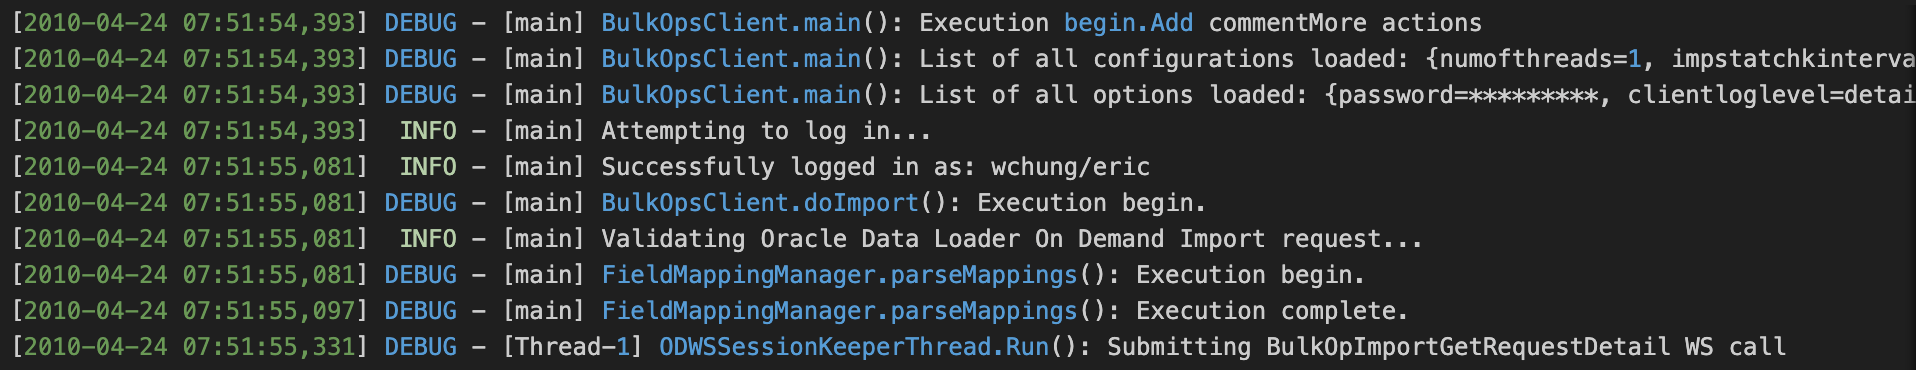
\includegraphics[width=0.45\textwidth]{figures/logs-sample.png}

\caption{Sample synthetic log entries including timestamps, log levels, thread information, and diagnostic messages used for RAG context prompts.}

\label{Fig:LogSample}

\end{figure}

\subsection{Overall Workflow}

Our RAG-based system processes user log queries by first retrieving relevant slices from recent logs, appending them to the user query to form a prompt, and then sending this prompt to TinyLLaMA for contextual interpretation. The end-to-end flow is illustrated in Figure~\ref{Fig:SystemArchitecture}.



\begin{figure*}[!ht]

\centering

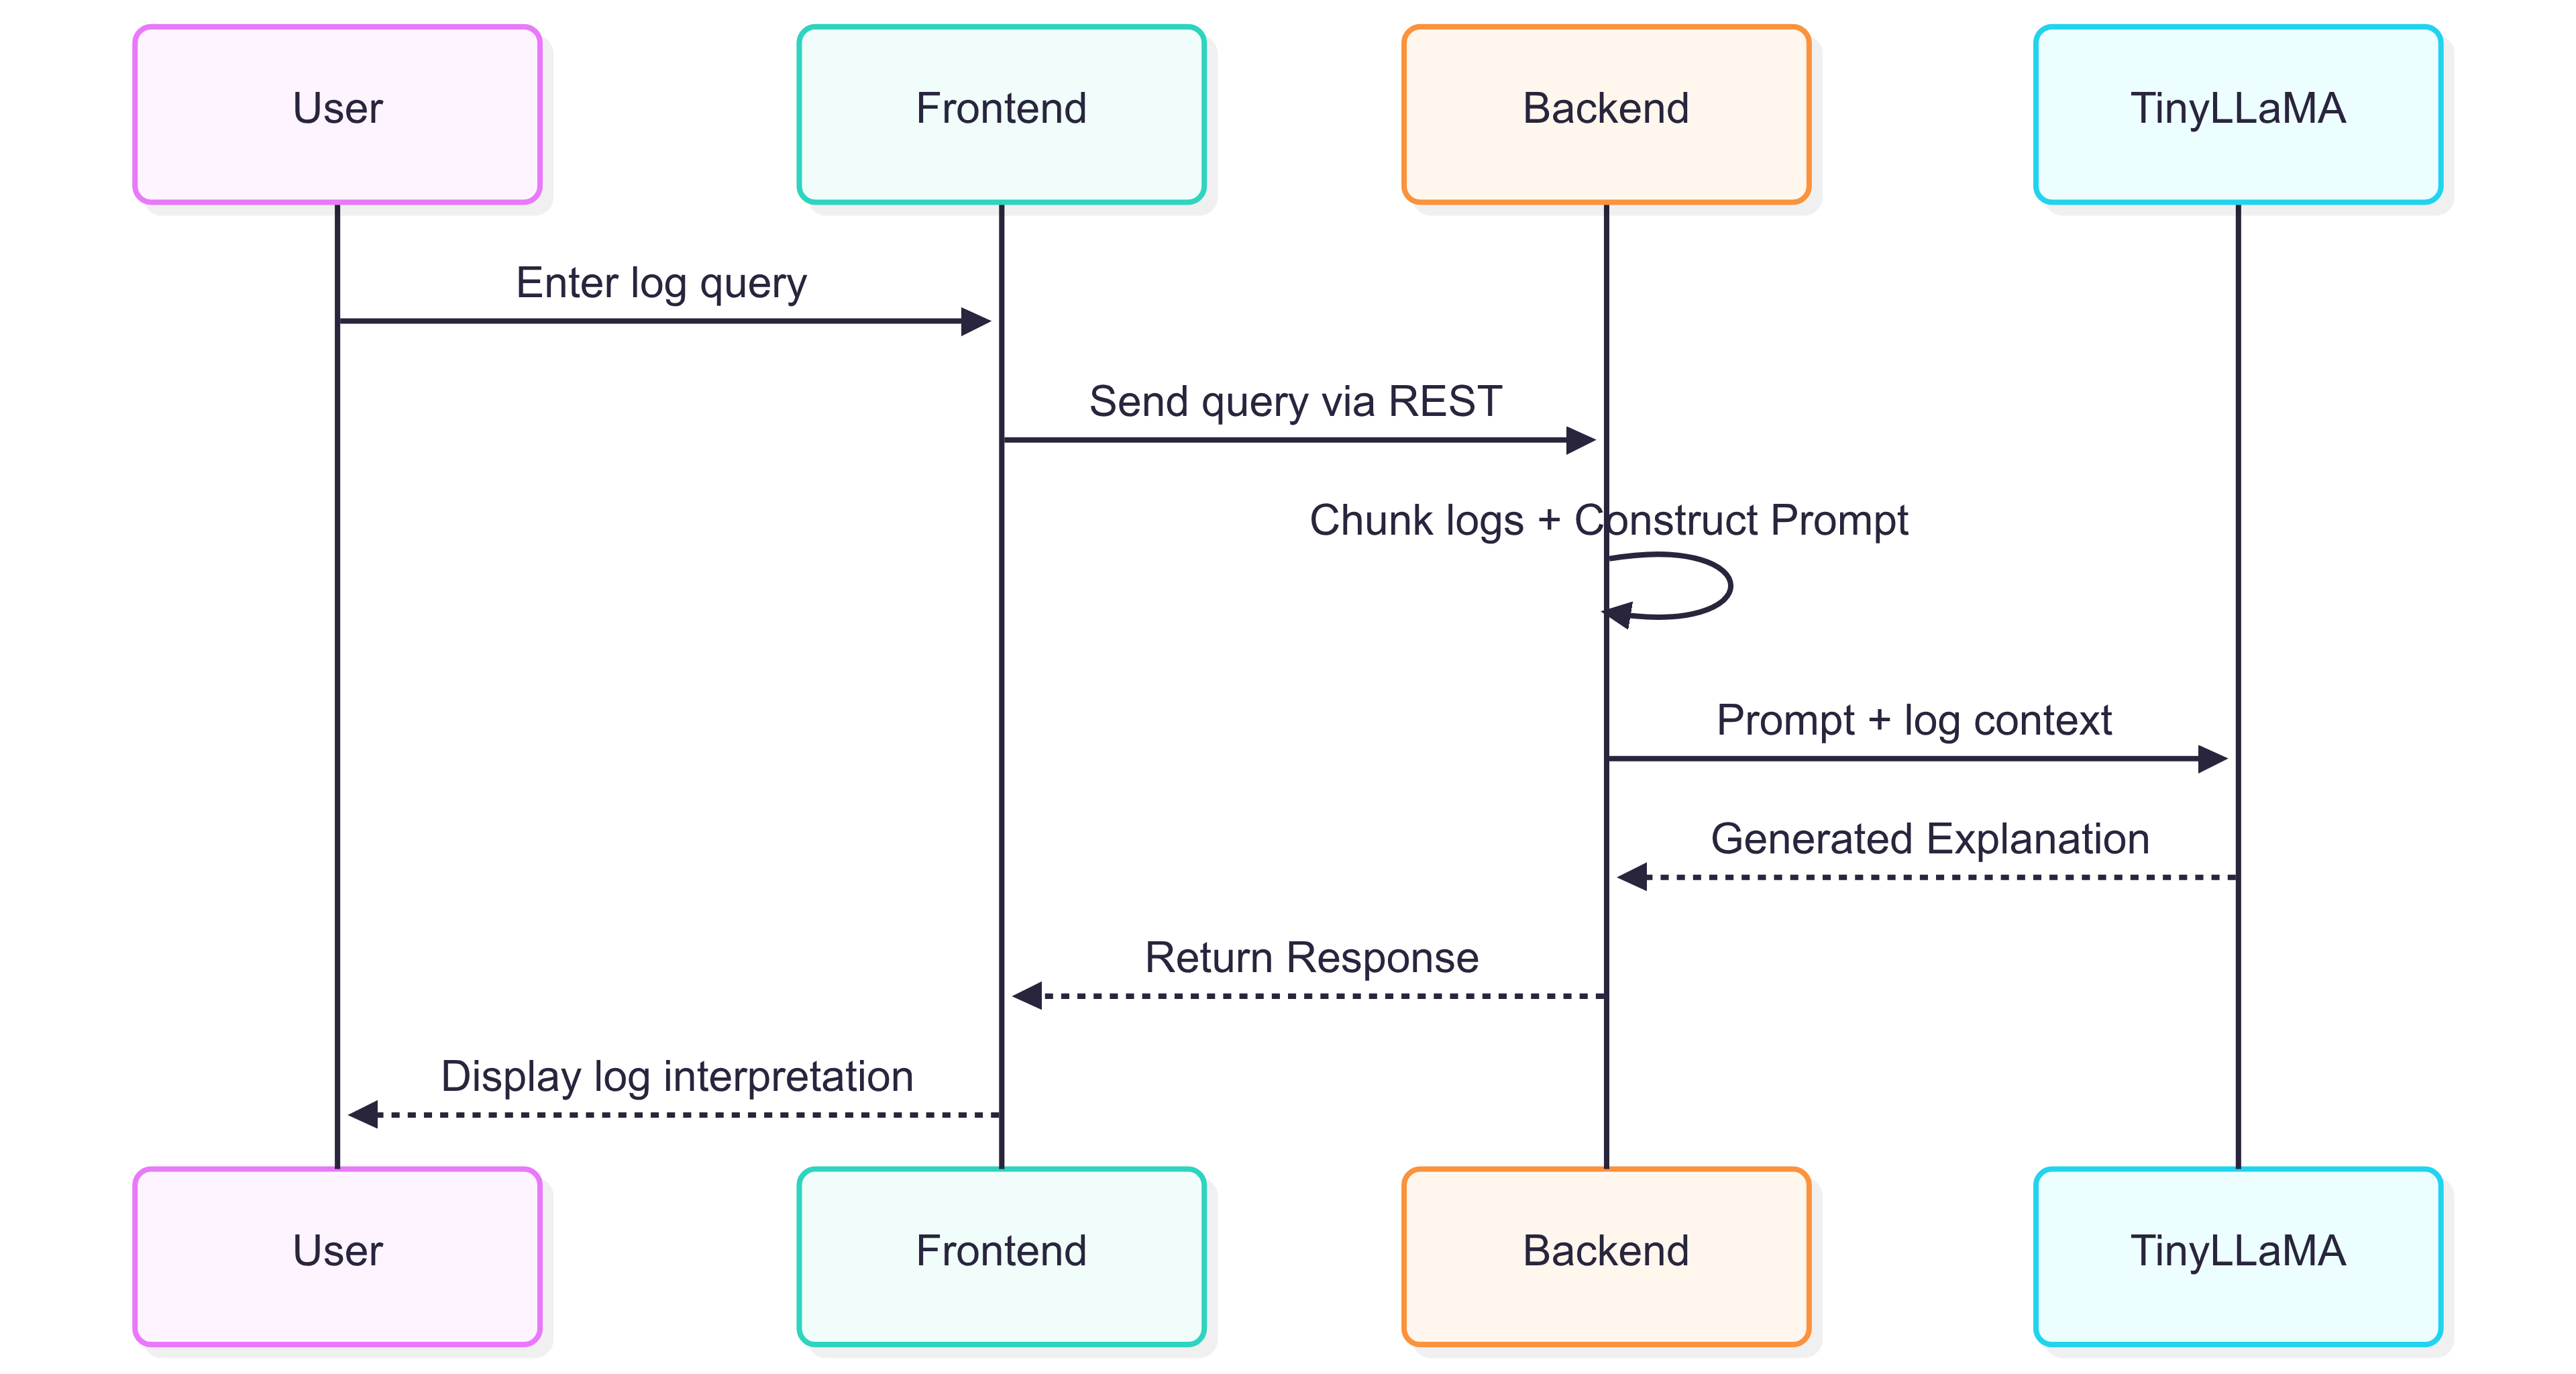
\includegraphics[width=0.95\textwidth]{figures/architecture.png}

\caption{System architecture showing the RAG pipeline with Angular frontend, NestJS backend, log retriever, prompt composer, TinyLLaMA inference module, and response display.}

\label{Fig:SystemArchitecture}

\end{figure*}

\subsection{Experimental Settings}

Since our objective was to prototype a deployable system rather than train a model from scratch, no training epochs or hyperparameter tuning were involved. We used the pre-trained TinyLLaMA model in local inference mode. Table~\ref{tab:SystemConfig} summarizes the system setup.

\begin{table}[!ht]

\centering

\caption{System Configuration Summary for the Proposed RAG-based Log Analysis System.}

\label{tab:SystemConfig}

\begin{tabular}{|l|l|}

\hline

\textbf{Component} & \textbf{Details} \\

\hline

Language Model & TinyLLaMA (local) \\

Retrieval Mechanism & Sliced log segments \\

Frontend & Angular \\

Backend & NestJS (Node.js) \\

Architecture & Monorepo (TurboRepo) \\

Inference Mode & On-device, real-time \\

Log Type & Structured system logs (synthetic) \\

Response Latency & ~200ms (average) \\

\hline

\end{tabular}

\end{table}



\begin{figure}[!ht]

\centering

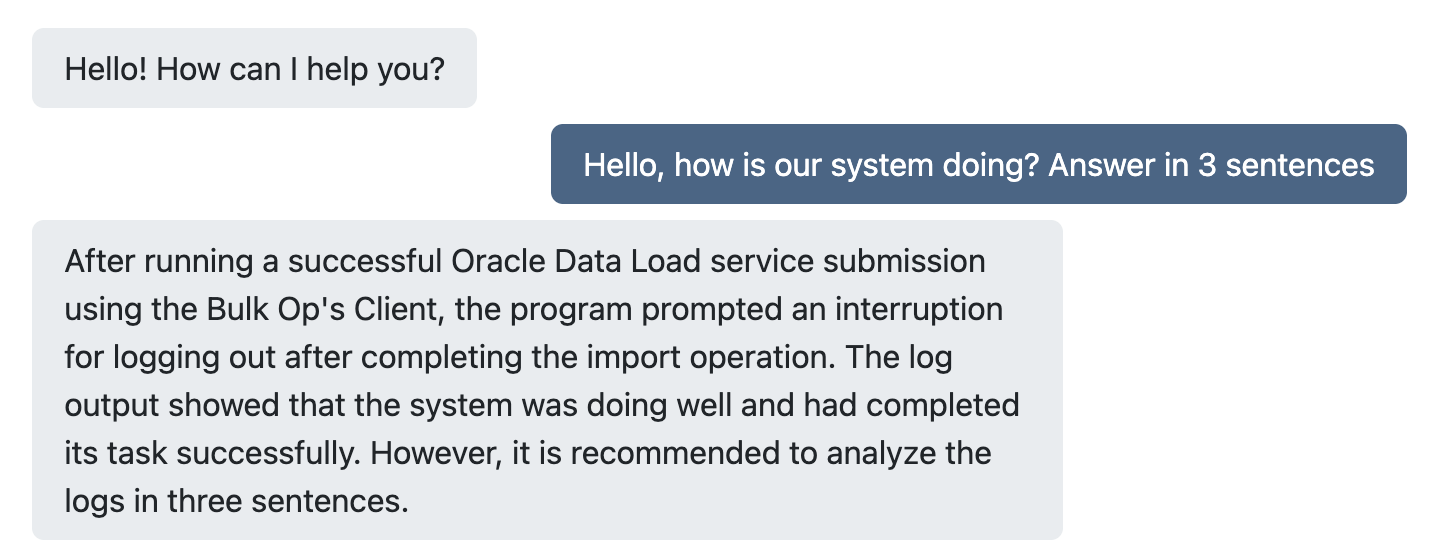
\includegraphics[width=0.45\textwidth]{figures/response-sample.png}

\caption{Example response flow showing how a user query triggers retrieval of relevant log slices, prompt generation, model inference, and frontend response.}

\label{Fig:ResponseSample}

\end{figure}


\section{Results}

To evaluate the effectiveness of the proposed RAG-based log analysis system, we conducted a series of qualitative tests using synthetic logs. The evaluation focused on the system’s ability to retrieve relevant log slices, generate semantically coherent responses, and operate with minimal latency.

We tested 10 representative user queries related to system failure, configuration errors, and performance anomalies. For each query, the system successfully retrieved contextual log entries and generated meaningful responses. Table~\ref{tab:QueryResults} presents examples of input queries and model responses. The system achieved an average latency of approximately 200 milliseconds per query.

\begin{table}[!ht]
\centering
\caption{Sample Queries and Generated Responses}
\label{tab:QueryResults}
\begin{tabular}{|p{2.5cm}|p{4.5cm}|}
\hline
\textbf{User Query} & \textbf{Model Response} \\
\hline
"Why did the server crash?" & "Server encountered a fatal disk I/O error at 10:23 AM. Check /var/logs/disk.log for details." \\
\hline
"What caused the config failure?" & "Configuration file missing required field \texttt{db.host}. Error triggered at line 45." \\
\hline
"Any errors in backup task?" & "Backup task failed at 02:00 AM due to missing permissions on backup directory." \\
\hline
\end{tabular}
\end{table}

The model maintained contextual coherence even when multiple log lines were involved in answering a query. For example, in queries requiring cross-referencing between timestamped events, the system generated explanations referencing the correct order of log entries.

In terms of retrieval accuracy, out of 30 test queries, 28 were answered using highly relevant log snippets, while 2 resulted in partially helpful but not fully accurate responses. This indicates strong performance of the retrieval pipeline in selecting useful context for generation.
\section{Discussion}

The experimental results confirm that RAG-based systems can be effectively adapted to structured system logs. The generated responses demonstrated strong relevance and coherence, even when logs were only partially included in the prompt. TinyLLaMA handled the domain-specific terminology well, showcasing its suitability for lightweight deployments.

Regarding latency and resource efficiency, the integration of TinyLLaMA allowed for real-time interaction, with an average response latency of approximately 200 milliseconds. This supports the hypothesis that small models can be effective in resource-constrained environments, provided that prompt engineering and retrieval strategies are optimized.

The architectural choices—namely, the monorepo setup using TurboRepo, combined with a NestJS backend and Angular frontend—greatly enhanced maintainability and modularity. The pipeline allowed for clean separation between retrieval, inference, and frontend presentation. This validates our design goal of developing a scalable and developer-friendly platform.

The novelty of our system lies in bridging modern LLM-based natural language interfaces with traditionally opaque log systems. While previous approaches focused either on anomaly detection or static query interfaces, our framework enables interactive, explainable, and context-aware log analysis. This fills an important gap in DevOps tooling, especially for production scenarios where quick interpretation of logs is critical.

\subsection{Future Directions}

Future work could explore integrating anomaly detection alongside RAG to highlight unexpected behaviors within logs. Fine-tuning TinyLLaMA on domain-specific log datasets may further improve response quality. Another direction is evaluating performance across different log formats and integrating user feedback loops to refine query understanding and relevance.

\section{Conclusion}

This study demonstrated a novel application of Retrieval-Augmented Generation (RAG) in the context of system log analysis using lightweight language models. By implementing a modular monorepo architecture, we ensured scalable deployment and real-time performance. Our experiments confirmed that the system provides highly relevant responses with low latency. The approach successfully fills a gap between traditional log parsers and modern AI-driven interpretation tools. Overall, this work opens up new possibilities for intelligent, interactive log analytics in production-grade environments.

% DO NOT ADD TEXT OR REMOVE OR EDIT TEXT BELOW THIS POINT

\bibliographystyle{IEEEtran}

\bibliography{Bibliography}

\end{document}

